\chapter{行列式}

行列式对于刚上大学的我们而言是一个全新的概念,但掌握行列式并不难,最重要的部分是行列式的计算,学习计算套路并做题巩固就能熟练解题。

学习本章的要求如下:

\begin{enumerate}
    \item 领会行列式的定义;
    \item 学会使用对角线法则计算2阶和3阶行列式;
    \item 代数余子式的定义和性质;
    \item 行列式按行(列)展开;
    \item 正确使用行列式的有关性质化简、计算行列式;
    \item 掌握使用Cramer法则判定线性方程组解的存在性、唯一性及求出方程组的解。
\end{enumerate}

\section{行列式的定义与性质}

\subsection{引入——二阶行列式与一类二元线性方程组的解}

在初等数学中,我们用代入消元法求解二元和三元线性方程组,可以看出,线性方程组的解完全由未知量的系数和常数项所确定。

为了更清楚地表达线性方程组解与未知量地系数和常数项地关系,我们在本章先引入二阶行列式的概念,并在二阶行列式的基础上,给出$n$阶行列式的定义并讨论其性质,进而把$n$阶行列式应用于$n$元线性方程组。

行列式是一种常用的数学工具,在数学及其它学科中都有着广泛的应用。

\begin{example}
    用消元法解二元线性方程组

    \begin{equation}
        \left\{
        \begin{array}{c}
            a_{11}x_1+a_{12}x_2=b_1 \\
            a_{21}x_1+a_{22}x_2=b_2
        \end{array}
        \right.\label{eq1.1}
    \end{equation}
\end{example}

\begin{solution}
    用加减消元法可得

    \begin{equation}
        \left\{
        \begin{array}{c}
            (a_{11}a_{22}-a_{12}a_{21})x_1=b_1a_{22}-a_{12}b_{2} \\
            (a_{11}a_{22}-a_{12}a_{21})x_2=a_{11}b_{2}-b_{1}a_{21}
        \end{array}
        \right.\label{eq1.2}
    \end{equation}

    当$a_{11}a_{22}-a_{12}a_{21}\ne  0$时,求得方程组的解为

    \begin{equation}
        \left\{
        \begin{array}{c}
            x_1=\frac{b_1a_{22}-a_{12}b_{2}}{a_{11}a_{22}-a_{12}a_{21}} \\
            x_2=\frac{a_{11}b_{2}-b_{1}a_{21}}{a_{11}a_{22}-a_{12}a_{21}}
        \end{array}
        \right.
    \end{equation}
\end{solution}

为了记忆该公式,引入记号

$$\left|\begin{array}{ccc}
        a_{11} & a_{12} \\
        a_{21} & a_{22}
    \end{array}\right| \xlongequal{\rm def} a_{11}a_{22}-a_{12}a_{21} $$

并称之为\textbf{二阶行列式},其中$a_{ij}$称为行列式的\textbf{元素},$a_{ij}$的两个下标表示该元素在行列式中的位置,第一个下标称为\textbf{行标},表示该元素所在的行,第二个下标称为\textbf{列标},表示该元素所在的列,常称$a_{ij}$为行列式的\textbf{$(i,j)$元素}或\textbf{元}。

由二阶行列式的定义,\ref{eq1.2}式中$x_1$,$x_2$ 的分子也可以写成二阶行列式,即

$$
    b_1a_{22}-a_{12}b_{2}= \left|\begin{array}{ccc}
        b_1 & a_{12} \\
        b_2 & a_{22}
    \end{array}\right| , a_{11}b_{2}-b_{1}a_{21}= \left|\begin{array}{ccc}
        a_{11} & b_1 \\
        a_{21} & b_2
    \end{array}\right|  \\
$$

若记$D= \left|\begin{array}{ccc}
        a_{11} & a_{12} \\
        a_{21} & a_{22}
    \end{array}\right| , D_1=\left|\begin{array}{ccc}
        b_1 & a_{12} \\
        b_2 & a_{22}
    \end{array}\right| ,D_2= \left|\begin{array}{ccc}
        a_{11} & b_1 \\
        a_{21} & b_2
    \end{array}\right|  $,

则当$D \ne 0 $时,方程组\ref{eq1.1}有唯一解\mn{$D$称为系数行列式,$D_{j}$是用常数项 $b_{1},b_{2}$替换$D$中的第 $j$列($j=1,2$)。}
$$
    x_1=\frac{D_1}{D},x_2=\frac{D_2}{D}
$$

\begin{example}
    计算二阶行列式
    $\left|\begin{array}{ccc}
            5 & -1 \\
            3 & 2
        \end{array}\right| $
\end{example}

\begin{solution}
    $\left|\begin{array}{ccc}
            5 & -1 \\
            3 & 2
        \end{array}\right| =5\times 2-(-1)\times 3=13$
\end{solution}

\begin{example}
    解二元线性方程组
    $
        \left\{
        \begin{array}{c}
            3x_1-2x_2=1 \\
            2x_1+x_2=3
        \end{array}
        \right.
    $
\end{example}

\begin{solution}
    因为$ D=\left|\begin{array}{ccc}
            3 & -2 \\
            2 & 1
        \end{array}\right| =7\ne 0 $,且$D_1=\left|\begin{array}{ccc}
            1 & -2 \\
            3 & 1
        \end{array}\right| =7 $,$D_2=\left|\begin{array}{ccc}
            3 & 1 \\
            2 & 3
        \end{array}\right| =7 $,

    所以方程组有唯一解为

    $$ x_1=\frac{D_1}{D}=1,x_2=\frac{D_2}{D}=1 $$
\end{solution}

\subsection{$n$阶行列式的定义}

\begin{definition}[$n$阶行列式]
    $n$阶行列式是由$n^2$个数$a_{ij}(i,j=1,2,\cdots,n)$排成$n$行、$n$列的算式

    $$D = \left|\begin{array}{ccccc}
            a_{11} & a_{12} & \cdots & a_{1n} \\
            a_{21} & a_{22} & \cdots & a_{2n} \\
            \vdots & \vdots &        & \vdots \\
            a_{n1} & a_{n2} & \cdots & a_{nn}
        \end{array}\right|$$
\end{definition}

\begin{remark}
    不要把一阶行列式$\left | a_{11} \right |$与$a_{11}$的绝对值相混淆。
\end{remark}

\begin{definition}[余子式和代数余子式]
    在$n$阶行列式$D$=det($a_{ij}$)中,称删去$a_{ij}$所在的第$i$行元素和第$j$列元素后由剩余元素按照它们原来的相对次序所形成的$n-1$阶行列式为$a_{ij}$的余子式,记为$M_{ij}$,而称

    $$
        A_{ij}=(-1)^{i+j}M_{ij}
    $$
    为$a_{ij}$的代数余子式。
\end{definition}

\begin{remark}
    行列式$D$的$(i,j)$元素的余子式和代数余子式都与$D$的第$i$行元素及$D$的第$j$列元素无关。
\end{remark}

\begin{example}
    已知三阶行列式
    $D=\left|\begin{array}{ccc}
            1  & x & 1  \\
            2  & 3 & -3 \\
            -3 & y & 4
        \end{array}\right| $,求元素$x$与$y$的代数余子式之和。
\end{example}
\begin{solution}
    元素$x$,$y$的代数余子式分别为

    $$A_{12}=(-1)^{1+2}\left|\begin{array}{ccccc}
            2  & -3 \\
            -3 & 4
        \end{array}\right|=1,A_{32}
        =(-1)^{3+2}
        \left|\begin{array}{ccccc}
            1 & 1  \\
            2 & -3
        \end{array}\right|=5
    $$

    所以,$A_{12}+A_{32}=6.$
\end{solution}

\subsubsection{对角线法则}

\begin{marginfigure}[3em]
	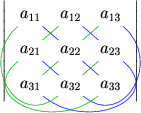
\includegraphics[width=\marginparwidth]{figures/对角线法则.png}
\end{marginfigure}

\begin{remark}
    对角线展开法则只适用于二阶及三阶行列式,它对四阶及四阶以上的行列式已不再适用。
\end{remark}
\begin{example}
    计算三阶行列式
    $D=\left|\begin{array}{ccc}
            1  & 2 & 3 \\
            -1 & 3 & 4 \\
            2  & 5 & 2
        \end{array}\right| $
\end{example}
\begin{solution}
    $ D=1\times 3\times 2 +2\times4\times2+3 \times (-1)\times 5 -3\times 3 \times2 -2\times (-1)\times 2 -1\times 4\times 5=-27$
\end{solution}

\begin{example}
    计算三阶行列式
    $\left|\begin{array}{ccc}
            a & b & c \\
            b & c & a \\
            c & a & b
        \end{array}\right| $
\end{example}
\begin{solution}
    $ \left|\begin{array}{ccc}
            a & b & c \\
            b & c & a \\
            c & a & b
        \end{array}\right|=abc+bca+cba-bbb-aaa-ccc=3abc-a^{3}-b^{3}-c^{3}$
\end{solution}

\begin{example}
    计算三阶行列式
    $ \left|\begin{array}{ccc}
            1     & 1     & 1     \\
            a     & b     & c     \\
            a^{2} & b^{2} & c^{2}
        \end{array}\right| $
\end{example}
\begin{solution}
    $ \left|\begin{array}{ccc}
            1     & 1     & 1     \\
            a     & b     & c     \\
            a^{2} & b^{2} & c^{2}
        \end{array}\right|=bc^{2}+ca^{2}+ab^{2}-ac^{2}-ba^{2}-cb^{2}=(a-b)(b-c)(c-a)$
\end{solution}

\subsubsection{上(下)三角行列式的性质}

下三角形行列式(主对角线上(下)边的元素全为零的行列式称为下(上)三角形行列式)

$$D_{n}= \left|\begin{array}{ccccc}
        a_{11} & 0      & 0      & \cdots & 0      \\
        a_{21} & a_{22} & 0      & \cdots & 0      \\
        a_{31} & a_{32} & a_{33} & \cdots & 0      \\
        \vdots & \vdots & \vdots & \ddots & \vdots \\
        a_{n1} & a_{n2} & a_{n3} & \cdots & a_{nn} \\
    \end{array}\right| =a_{11}a_{22}\cdots a_{nn}$$

即下三角形行列式的值等于它的主对角线元素之积.

副对角线上边的元素全为零的行列式

$$
    \left|\begin{array}{ccccc}
        0      & \cdots & 0         & 0         & a_{1n} \\
        0      & \cdots & 0         & a_{2,n-1} & a_{2n} \\
        0      & \cdots & a_{3,n-2} & a_{3,n-1} & a_{3n} \\
        \vdots & \ddots & \vdots    & \vdots    & \vdots \\
        a_{n1} & \cdots & a_{n,n-2} & a_{n,n-1} & a_{nn} \\
    \end{array}\right| =\textcolor{red}{(-1)^{\frac{n(n-1)}{2}}}a_{1n}a_{2,n-1}\cdots a_{n1}$$


\subsection{行列式的基本性质}

行列式的基本性质非常重要,是后面简化行列式计算的基础,理解并推导每一条性质,才能加深记忆并熟练运用到题目中。

\begin{property}
    行列式与它的转置行列式相等,即$D=D^{T}$。
\end{property}

\begin{property}
    互换行列式两列的位置,行列式的值反号。
\end{property}

\begin{property}
    行列式$D$等于它的任一行元素分别与其对应的代数余子式的乘积之和,即
    $$ D=a_{i1}A_{i1}+a_{i2}A_{i2} +\cdots +a_{in}A_{in}= \sum_{j=1}^{n}a_{ij}A_{ij},  i=1,2,\cdots,n.
    $$

    并称该式为行列式按第$i$行展开的公式。
\end{property}

这一性质即行列式的\textcolor{magenta}{按行(列)展开法则},利用这一法则并结合行列式性质,可以简化行列式计算。

\begin{example}
    求解$a$,$b$为何值时
    $ \left|\begin{array}{ccc}
            a  & b & 0 \\
            -b & a & 0 \\
            1  & 0 & 1
        \end{array}\right| =0 $
\end{example}
\begin{solution}
    行列式按最后一行展开得

    $$ \left|\begin{array}{ccc}
            a  & b & 0 \\
            -b & a & 0 \\
            1  & 0 & 1
        \end{array}\right| =a^{2}+b^{2} =0$$

    所以$a=b=0$时,给定的行列式为零。
\end{solution}

\begin{example}[课后题6.(2)]
    计算行列式
    $ \left|\begin{array}{cccccc}
            x      & y      & 0      & \cdots & 0      & 0      \\
            0      & x      & y      & \cdots & 0      & 0      \\
            \vdots & \vdots & \vdots & \ddots & \vdots & \vdots \\
            0      & 0      & 0      & \cdots & x      & y      \\
            y      & 0      & 0      & \cdots & 0      & x
        \end{array}\right|  $
\end{example}

\begin{solution}
    根据行列式的特点,对第一列用性质1.1.3展开可得

    $
        \left|\begin{array}{cccccc}
            x      & y      & 0      & \cdots & 0      & 0      \\
            0      & x      & y      & \cdots & 0      & 0      \\
            \vdots & \vdots & \vdots & \ddots & \vdots & \vdots \\
            0      & 0      & 0      & \cdots & x      & y      \\
            y      & 0      & 0      & \cdots & 0      & x
        \end{array}\right| =
        x\left|\begin{array}{cccccc}
            x      & y      & \cdots & 0      & 0      \\
            \vdots & \vdots & \ddots & \vdots & \vdots \\
            0      & 0      & \cdots & x      & y      \\
            0      & 0      & \cdots & 0      & x
        \end{array}\right|+(-1)^{n+1}y
        \left|\begin{array}{cccccc}
            y      & 0      & \cdots & 0      & 0      \\
            x      & y      & \cdots & 0      & 0      \\
            \vdots & \vdots & \ddots & \vdots & \vdots \\
            0      & 0      & \cdots & x      & y
        \end{array}\right|\\
        =x^{n}+(-1)^{n+1}y^{n}
    $
\end{solution}

\begin{tuilun}
    若行列式$D$的某行元素全为零,则$D=0$。
\end{tuilun}

\begin{property}
    若行列式某行的各元素有公因子$k$则可将$k$提到行列式符号
    外边来(或者说,用一个数$k$去乘行列式,就等于用$k$去乘行列式某行的每个元素)即

    $$\left|\begin{array}{ccccc}
            a_{11}  & a_{12}  & \cdots & a_{1n}  \\
            \vdots  & \vdots  & \ddots & \vdots  \\
            ka_{i1} & ka_{i2} & \cdots & ka_{in} \\
            \vdots  & \vdots  & \ddots & \vdots  \\
            a_{n1}  & a_{n2}  & \cdots & a_{nn}
        \end{array}\right| =  k \left|\begin{array}{ccccc}
            a_{11} & a_{12} & \cdots & a_{1n} \\
            \vdots & \vdots & \ddots & \vdots \\
            a_{i1} & a_{i2} & \cdots & a_{in} \\
            \vdots & \vdots & \ddots & \vdots \\
            a_{n1} & a_{n2} & \cdots & a_{nn}
        \end{array}\right|  $$
\end{property}

\begin{example}
    计算三阶行列式
    $ \left|\begin{array}{cccc}
            4 & 1 & 1 & 1 \\
            1 & 4 & 1 & 1 \\
            1 & 1 & 4 & 1 \\
            1 & 1 & 1 & 4
        \end{array}\right| $
\end{example}

\begin{solution}
    这个行列式的特点是各列4个数之和都是7,所以有
    \small
    $ \left|\begin{array}{cccc}
            4 & 1 & 1 & 1 \\
            1 & 4 & 1 & 1 \\
            1 & 1 & 4 & 1 \\
            1 & 1 & 1 & 4
        \end{array}\right|
        % \xlongequal[]{}
        \xlongequal{\substack{r_{21}(1),\\r_{31}(1),\\r_{41}(1)}}
        \left|\begin{array}{cccc}
            7 & 7 & 7 & 7 \\
            1 & 4 & 1 & 1 \\
            1 & 1 & 4 & 1 \\
            1 & 1 & 1 & 4
        \end{array}\right| =7
        \left|\begin{array}{cccc}
            1 & 1 & 1 & 1 \\
            1 & 4 & 1 & 1 \\
            1 & 1 & 4 & 1 \\
            1 & 1 & 1 & 4
        \end{array}\right|
        \xlongequal{\substack{r_{12}(-1),\\ r_{13}(-1),\\r_{14}(-1)}}
        \left|\begin{array}{cccc}
            1 & 1 & 1 & 1 \\
            0 & 3 & 0 & 0 \\
            0 & 0 & 3 & 0 \\
            0 & 0 & 0 & 3
        \end{array}\right| =189.$
\end{solution}

\begin{property}
    若行列式某行的每个元素都是两个数的和,则可将此行列式写
    成两个行列式的和:
    \small
    $$\left|\begin{array}{ccccc}
            a_{11}        & a_{12}        & \cdots & a_{1n}        \\
            \vdots        & \vdots        & \ddots & \vdots        \\
            a_{i1}+b_{i1} & a_{i2}+b_{i2} & \cdots & a_{in}+b_{in} \\
            \vdots        & \vdots        & \ddots & \vdots        \\
            a_{n1}        & a_{n2}        & \cdots & a_{nn}
        \end{array}\right|   =   \left|\begin{array}{ccccc}
            a_{11} & a_{12} & \cdots & a_{1n} \\
            \vdots & \vdots & \ddots & \vdots \\
            a_{i1} & a_{i2} & \cdots & a_{in} \\
            \vdots & \vdots & \ddots & \vdots \\
            a_{n1} & a_{n2} & \cdots & a_{nn}
        \end{array}\right| +\left|\begin{array}{ccccc}
            a_{11} & a_{12} & \cdots & a_{1n} \\
            \vdots & \vdots & \ddots & \vdots \\
            b_{i1} & b_{i2} & \cdots & b_{in} \\
            \vdots & \vdots & \ddots & \vdots \\
            a_{n1} & a_{n2} & \cdots & a_{nn}
        \end{array}\right|   $$
\end{property}

\begin{example}
    计算行列式
    $ \left|\begin{array}{cccc}
            3   & 1   & 1  \\
            297 & 101 & 99 \\
            5   & -3  & 2
        \end{array}\right|$.
\end{example}

\begin{solution}
    根据行列式的性质有

    $ \left|\begin{array}{cccc}
            3   & 1   & 1  \\
            297 & 101 & 99 \\
            5   & -3  & 2
        \end{array}\right|=
        \left|\begin{array}{cccc}
            3     & 1     & 1     \\
            300-3 & 100+1 & 100-1 \\
            5     & -3    & 2
        \end{array}\right|=
        \left|\begin{array}{cccc}
            3   & 1   & 1   \\
            300 & 100 & 100 \\
            5   & -3  & 2
        \end{array}\right|+
        \left|\begin{array}{cccc}
            3  & 1  & 1  \\
            -3 & 1  & -1 \\
            5  & -3 & 2
        \end{array}\right|
        = 0+\left|\begin{array}{cccc}
            3  & 1  & 1  \\
            -3 & 1  & -1 \\
            5  & -3 & 2
        \end{array}\right|
        \overset{r_{12(1)}}{=}
        \left|\begin{array}{cccc}
            3 & 1  & 1 \\
            0 & 2  & 0 \\
            5 & -3 & 2
        \end{array}\right|=12-10=2.$
\end{solution}


\begin{property}
    若行列式$D$中有两行的对应元素都相等,则$D=0$。
\end{property}

\begin{example}
    证明
    $$ \left|\begin{array}{cccc}
            a_{1}+b_{1} & b_{1}+c_{1} & c_{1}+a_{1} \\
            a_{2}+b_{2} & b_{2}+c_{2} & c_{2}+a_{2} \\
            a_{3}+b_{3} & b_{3}+c_{3} & c_{3}+a_{3}
        \end{array}\right|=2
        \left|\begin{array}{cccc}
            a_{1} & b_{1} & c_{1} \\
            a_{2} & b_{2} & c_{2} \\
            a_{3} & b_{3} & c_{3}
        \end{array}\right|
    $$
\end{example}

\begin{solution}
    根据行列式的性质有

    $
        \left|\begin{array}{cccc}
            a_{1}+b_{1} & b_{1}+c_{1} & c_{1}+a_{1} \\
            a_{2}+b_{2} & b_{2}+c_{2} & c_{2}+a_{2} \\
            a_{3}+b_{3} & b_{3}+c_{3} & c_{3}+a_{3}
        \end{array}\right|=
        \left|\begin{array}{cccc}
            a_{1} & b_{1}+c_{1} & c_{1}+a_{1} \\
            a_{2} & b_{2}+c_{2} & c_{2}+a_{2} \\
            a_{3} & b_{3}+c_{3} & c_{3}+a_{3}
        \end{array}\right|+
        \left|\begin{array}{cccc}
            b_{1} & b_{1}+c_{1} & c_{1}+a_{1} \\
            b_{2} & b_{2}+c_{2} & c_{2}+a_{2} \\
            b_{3} & b_{3}+c_{3} & c_{3}+a_{3}
        \end{array}\right|
    $

    又因为
    $$\left|\begin{array}{cccc}
            a_{1} & b_{1}+c_{1} & c_{1}+a_{1} \\
            a_{2} & b_{2}+c_{2} & c_{2}+a_{2} \\
            a_{3} & b_{3}+c_{3} & c_{3}+a_{3}
        \end{array}\right|
        \xlongequal{c_{13}(-1)}\left|\begin{array}{cccc}
            a_{1} & b_{1}+c_{1} & c_{1} \\
            a_{2} & b_{2}+c_{2} & c_{2} \\
            a_{3} & b_{3}+c_{3} & c_{3}
        \end{array}\right|
        \xlongequal{c_{32}(-1)}\left|\begin{array}{cccc}
            a_{1} & b_{1} & c_{1} \\
            a_{2} & b_{2} & c_{2} \\
            a_{3} & b_{3} & c_{3}
        \end{array}\right|
    $$

    $$\left|\begin{array}{cccc}
            b_{1} & b_{1}+c_{1} & c_{1}+a_{1} \\
            b_{2} & b_{2}+c_{2} & c_{2}+a_{2} \\
            b_{3} & b_{3}+c_{3} & c_{3}+a_{3}
        \end{array}\right|
        \xlongequal{c_{12}(-1)}\left|\begin{array}{cccc}
            b_{1} & c_{1} & c_{1}+a_{1} \\
            b_{2} & c_{2} & c_{2}+a_{2} \\
            b_{3} & c_{3} & c_{3}+a_{3}
        \end{array}\right|
        \xlongequal{c_{23}(-1)}\left|\begin{array}{cccc}
            b_{1} & c_{1} & a_{1} \\
            b_{2} & c_{2} & a_{2} \\
            b_{3} & c_{3} & a_{3}
        \end{array}\right|
        \xlongequal{\substack{c_{32}, //c_{21}}}\left|\begin{array}{cccc}
            a_{1} & b_{1} & c_{1} \\
            a_{2} & b_{2} & c_{2} \\
            a_{3} & b_{3} & c_{3}
        \end{array}\right|
    $$

    所以
    $$ \left|\begin{array}{cccc}
            a_{1}+b_{1} & b_{1}+c_{1} & c_{1}+a_{1} \\
            a_{2}+b_{2} & b_{2}+c_{2} & c_{2}+a_{2} \\
            a_{3}+b_{3} & b_{3}+c_{3} & c_{3}+a_{3}
        \end{array}\right|=2
        \left|\begin{array}{cccc}
            a_{1} & b_{1} & c_{1} \\
            a_{2} & b_{2} & c_{2} \\
            a_{3} & b_{3} & c_{3}
        \end{array}\right|
    $$

\end{solution}

由性质 1.1.4 和性质 1.1.6,立即可得
\begin{tuilun}
    若行列式$D$中有两行的元素对应成比例,则$D=0$。
\end{tuilun}

利用性质 1.1.5 和推论 1.1.2,立即可得

\begin{property}
    把行列式某行的$k$倍加到另一行上去(指某行每个元素乘以常
    数$k$后加到另一行的对应元素上去),行列式的值不变,即????
\end{property}

\begin{remark}
    在这个变换中,只有第$j$行变了,第$i$行没有改变。
\end{remark}

性质 1.1.7 是一条很重要的性质.读者在下节将看到,在行列式的计算中,常常利用这条性质将行列式中的某些元素化为零,以便简化计算。

\begin{property}
    行列式$D$的任一行各元素分别与另一行对应元素的代数余子式的乘积之和等于零,即
    $$ a_{i1}A_{k1}+a_{i2}A_{k2} +\cdots +a_{in}A_{kn}= 0,  i\ne k.  $$
\end{property}


\section{行列式的计算}

上一节中简要通过例题介绍了利用行列式的性质对行列式进行简化计算,这一小节通过归纳出的方法和例题来帮助大家更系统掌握行列式的计算,解题中需要综合运用行列式的计算。
\subsection{定义法}

当行列式中零元素较多时可利用定义计算,按照某一行或某一列展开。

\begin{example}
    计算行列式

$$D_{n}= \left|\begin{array}{ccccc}
        0      & \cdots & 0      & 1      & 0      \\
        0      & \cdots & 2      & 0      & 0      \\
        \vdots & \ddots   & \vdots & \vdot    s & \vdots \\
        n-1    & \cdots & 0      & 0      & 0      \\
        0      & \cdots & 0      & 0      & n      \\
    \end{array}\right|$$
\end{example}
\begin{solution}
    将行列式按最后一行展开,由对角行列式的性质得

$$D_{n}=n \left|\begin{array}{cccc}
        0      & \cdots & 0      & 1      \\
        0      & \cdots & 2      & 0      \\
        \vdots &        & \vdots & \vdots \\
        n-1    & \cdots & 0      & 0
    \end{array}\right|=(-1)^{\frac{(n-1)(n-2)}{2}}n!$$
\end{solution}

\subsection{利用行列式的性质计算}

\begin{example}
    一个$n$阶行列式$D_{n}=\left |a_{ij} \right |$的元素满足$a_{ij}=-a_{ji},i,j=1,2,\cdots,n,$则称$D_{n}$为反对称行列式,证明:奇数阶反对称行列式为零。
\end{example}

\begin{proof}
    由$a_{ij}=-a_{ji}$知$a_{ii}=-a_{ii}$,即
$a_{ii}=0,i=1,2,\cdots,n$

故行列式$D_{n}$可表示为


$$D_{n}= \left|\begin{array}{cccccc}
        0       & a_{12}  & a_{13}  & \cdots & a_{1n} \\
        -a_{12} & 0       & a_{23}  & \cdots & a_{2n} \\
        -a_{13} & -a_{23} & 0       & \cdots & a_{3n} \\
        \vdots  & \vdots  & \vdots  &        & \vdots \\
        -a_{1n} & -a_{2n} & -a_{3n} & \cdots & 0
    \end{array}\right|$$

由行列式的性质$\left | A \right |=\left | A^{T} \right |$得

$$D_{n}= \left|\begin{array}{cccccc}
        0      & -a_{12} & -a_{13} & \cdots & -a_{1n} \\
        a_{12} & 0       & -a_{23} & \cdots & -a_{2n} \\
        a_{13} & a_{23}  & 0       & \cdots & -a_{3n} \\
        \vdots & \vdots  & \vdots  &        & \vdots  \\
        a_{1n} & a_{2n}  & a_{3n}  & \cdots & 0
    \end{array}\right|=(-1)^{n}
    \left|\begin{array}{cccccc}
        0       & a_{12}  & a_{13}  & \cdots & a_{1n} \\
        -a_{12} & 0       & a_{23}  & \cdots & a_{2n} \\
        -a_{13} & -a_{23} & 0       & \cdots & a_{3n} \\
        \vdots  & \vdots  & \vdots  &        & \vdots \\
        -a_{1n} & -a_{2n} & -a_{3n} & \cdots & 0
    \end{array}\right|=(-1)^{n}D_{n}
$$

当$n$为奇数时,得$D_{n}=-D_{n}$,因而得$D_{n}=0$。
\end{proof}

\subsection{化为三角形行列式}

若能把一个行列式经过适当变换化成三角形,其结果为行列式主对角线上元素的乘积。因此化三角形是行列式计算中的一个重要方法。

\begin{example}
    计算$n$阶行列式
$$D=\left|\begin{array}{cccccc}
        a      & b      & b      & \cdots & b      \\
        b      & a      & b      & \cdots & b      \\
        b      & b      & a      & \cdots & b      \\
        \vdots & \vdots & \vdots &        & \vdots \\
        b      & b      & b      & \cdots & a
    \end{array}\right|$$
\end{example}

\begin{solution}
    这个行列式的特点是每行(列)元素的和均相等,根据行列式的性质,把第2,3,...,$n$列都加到第1列上,行列式不变,得

$D=\left|\begin{array}{cccccc}
        a+(n-1)b & b      & b      & \cdots & b      \\
        a+(n-1)b & a      & b      & \cdots & b      \\
        a+(n-1)b & b      & a      & \cdots & b      \\
        a+(n-1)b & \vdots & \vdots &        & \vdots \\
        a+(n-1)b & b      & b      & \cdots & a
    \end{array}\right|
    =[a+(n-1)b]\left|\begin{array}{cccccc}
        1 & b      & b      & \cdots & b      \\
        1 & a      & b      & \cdots & b      \\
        1 & b      & a      & \cdots & b      \\
        1 & \vdots & \vdots &        & \vdots \\
        1 & b      & b      & \cdots & a
    \end{array}\right| \\
    =[a+(n-1)b]\left|\begin{array}{cccccc}
        1 & b      & b      & \cdots & b      \\
        0 & a-b    & 0      & \cdots & 0      \\
        0 & 0      & a-b    & \cdots & 0      \\
        0 & \vdots & \vdots &        & \vdots \\
        0 & 0      & 0      & \cdots & a-b
    \end{array}\right|
    =[a+(n-1)b](a-b)^{n-1}
$
\end{solution}

\subsection{降阶法}
降阶法是按某一行(或一列)展开行列式,这样可以降低一阶,更一般地是用拉普拉斯定理,这样可以降低多阶,为了使运算更加简便,往往是先利用行列式的性质化简,使行列式中有较多的零出现,然后再展开。

\begin{example}
    计算行列式

$$D=\left|\begin{array}{cccccc}
        a  & 1  & 0  & 0 \\
        -1 & b  & 1  & 0 \\
        0  & -1 & c  & 1 \\
        0  & 0  & -1 & d
    \end{array}\right|$$
\end{example}

\begin{solution}
    \small
$D\overset{r_{21}(a)}{=}\left|\begin{array}{cccccc}
        0  & 1+ab & a  & 0 \\
        -1 & b    & 1  & 0 \\
        0  & -1   & c  & 1 \\
        0  & 0    & -1 & d
    \end{array}\right|
    =(-1)(-1)^{2+1}\left|\begin{array}{cccccc}
        1+ab & a  & 0 \\
        -1   & c  & 1 \\
        0    & -1 & d
    \end{array}\right|
    \overset{c_{23}(d)}{=}\left|\begin{array}{cccccc}
        1+ab & a  & ad   \\
        -1   & c  & 1+cd \\
        0    & -1 & 0
    \end{array}\right|  \\
    =(-1)(-1)^{3+2}\left|\begin{array}{cccccc}
        1+ab & ad   \\
        -1   & 1+cd
    \end{array}\right|=abcd+ab+cd+ad+1
$
\end{solution}
\subsection{递推公式法}

递推公式法:对$n$阶行列式$D_{n}$找出$D_{n}$与$D_{n-1}$或$D_{n}$与$D_{n-1}$, $D_{n-2}$之间的一种关系——称为递推公式(其中$D_{n}$, $D_{n-1}$,$D_{n-2}$等结构相同),再由递推公式求出$D_{n}$的方法称为递推公式法。

\begin{example}
    证明

$$D_{n}=\left|\begin{array}{cccccc}
        x      & -1      & 0       & \cdots & 0      & 0       \\
        0      & x       & -1      & \cdots & 0      & 0       \\
        \vdots & \vdots  & \vdots  &        & \vdots           \\
        0      & 0       & 0       & \cdots & x      & -1      \\
        a_{n}  & a_{n-1} & a_{n-2} & \cdots & a_{2}  & a_{1}+x
    \end{array}\right|
    =x^{n}+a_{1}x^{n-1}+a_{2}x^{n-2}+\cdots+a_{n-1}x+a_{n},(n\ge 2)
$$
\end{example}

\begin{proof}
    将$D_{n}$按第1列展开得

$$D_{n}=x\left|\begin{array}{cccccc}
        x       & -1      & 0       & \cdots & 0      & 0       \\
        0       & x       & -1      & \cdots & 0      & 0       \\
        \vdots  & \vdots  & \vdots  &        & \vdots & \vdots  \\
        0       & 0       & 0       & \cdots & x      & -1      \\
        a_{n-1} & a_{n-2} & a_{n-3} & \cdots & a_{2}  & a_{1}+x
    \end{array}\right| +
    (-1)^{n+1}a_{n}\left|\begin{array}{cccccc}
        -1     & 0      & \cdots & 0      & 0  \\
        x      & -1     & \cdots & 0      & 0  \\
        \vdots & \vdots &        & \vdots      \\
        0      & 0      & \cdots & x      & -1
    \end{array}\right| \\
    =a_{n}+xD_{n-1}
$$

由此得递推公式:$D_{n}=a_{n}+xD_{n-1}$,利用此递推公式可得

$D_{n}=a_{n}+xD{n-1}=a_{n}+x(a_{n-1}+xD_{n-2})=a_{n}+a_{n-1}x+x^{2}D_{n-2}=\cdots=a_{n}+a_{n-1}x+\cdots+a_{1}x^{n-1}+x^{n}
$
\end{proof}

\subsection{利用范德蒙行列式}

\begin{example}
    计算行列式

$$D=\left|\begin{array}{cccccc}
        1                       & 1                       & \cdots & 1                       \\
        x_{1}+1                 & x_{2}+1                 & \cdots & x_{n}+1                 \\
        x_{1}^{2}+x_{1}         & x_{2}^{2}+x_{2}         & \cdots & x_{n}^{2}+x_{n}         \\
        \vdots                  & \vdots                  &        & \vdots                  \\
        x_{1}^{n-1}+x_{1}^{n-2} & x_{2}^{n-1}+x_{2}^{n-2} & \cdots & x_{n}^{n-1}+x_{n}^{n-2}
    \end{array}\right|$$
\end{example}

\begin{solution}
    把第$1$行的$-1$倍加到第$2$行,把新的第$2$行的$-1$倍加到第3行,以此类推直到把新的第$n-1$行的$-1$倍加到第$n$行,便得范德蒙行列式

$$D=\left|\begin{array}{cccccc}
        1           & 1           & \cdots & 1           \\
        x_{1}       & x_{2}       & \cdots & x_{n}       \\
        x_{1}^{2}   & x_{2}^{2}   & \cdots & x_{n}^{2}   \\
        \vdots      & \vdots      &        & \vdots      \\
        x_{1}^{n-1} & x_{2}^{n-1} & \cdots & x_{n}^{n-1}
    \end{array}\right|=\prod_{n\ge i > j\ge 1}^{} (x_{i}-x_{j})
$$
\end{solution}

\begin{example}
    计算$n+1$阶行列式

$$D=\left|\begin{array}{ccccccc}
        a_{1}^{n}   & a_{1}^{n-1}b_{1}     & a_{1}^{n-2}b_{1}^{2}     & \cdots & a_{1}b_{1}^{n-1}     & b_{1}^{n}   \\
        a_{2}^{n}   & a_{2}^{n-1}b_{2}     & a_{2}^{n-2}b_{2}^{2}     & \cdots & a_{2}b_{2}^{n-1}     & b_{2}^{n}   \\
        \vdots      & \vdots               & \vdots                   &        & \vdots               & \vdots      \\
        a_{n+1}^{n} & a_{n+1}^{n-1}b_{n+1} & a_{n+1}^{n-2}b_{n+1}^{2} & \cdots & a_{n+1}b_{n+1}^{n-1} & b_{n+1}^{n} \\
    \end{array}\right|$$

其中,$a_{1},a_{2},\cdots,a_{n+1} \neq 0$。
\end{example}

\begin{solution}
    这个行列式的每一行元素的形状都是$a_{i}^{n-k}b_{i}^{k},k=0,1,2,...,n.$ 即$a_{i}$按降幂排列,$b_{i}$按升幂排列,且次数之和都是$n$,又因$a_{i}\ne 0$,若在第i行($1,2,...,n$)提出公因子$a_{i}^{n}$,则$D$可化为一个转置的范德蒙行列式,即
    \small
$$
    D=a_{1}^{n}a_{2}^{n}\cdots a_{n+1}^{n}
    \left|\begin{array}{cccccc}
        1      & \frac{b_{1}}{a_{1}}     & (\frac{b_{1}}{a_{1}})^{2}     & \cdots & (\frac{b_{1}}{a_{1}})^{n}     \\
        1      & \frac{b_{2}}{a_{2}}     & (\frac{b_{2}}{a_{2}})^{2}     & \cdots & (\frac{b_{2}}{a_{2}})^{n}     \\
        \vdots & \vdots                  & \vdots                        &        & \vdots                        \\
        1      & \frac{b_{n+1}}{a_{n+1}} & (\frac{b_{n+1}}{a_{n+1}})^{2} & \cdots & (\frac{b_{n+1}}{a_{n+1}})^{n} \\
    \end{array}\right|
    =\prod_{i=1}^{n+1} a_{i}^{n}\prod_{1\le j< i\le n+1}^{} (\frac{b_{i}}{a_{i}}-\frac{b_{j}}{a_{j}})
    =\prod_{1\le j< i\le n+1}^{}(b_{i}a_{j}-a_{i}b_{j})
$$
\end{solution}

\subsection{加边法(升阶法)}

加边法(又称升阶法)是在原行列式中增加一行一列,且保持原行列式不变的方法。

\begin{example}
    计算$n$阶行列式

$$D_{n}=\left|\begin{array}{ccccccc}
        x+a_{1} & a_{2}   & \cdots & a_{n}   \\
        a_{1}   & x+a_{2} & \cdots & a_{n}   \\
        a_{1}   & a_{2}   & \cdots & a_{n}   \\
        \vdots  & \vdots  &        & \vdots  \\
        a_{1}   & a_{2}   & \cdots & x+a_{n}
    \end{array}\right|$$
\end{example}

\begin{solution}
    给行列式添上一行一列,行列式大小不变。

$ D_{n}=\left|\begin{array}{ccccccc}
        1      & a_{1} & \cdots & a_{n} \\
        0      &       &        &       \\
        \vdots &       & D_{n}  &       \\
        0      &       &        &
    \end{array}\right|
    \xlongequal[i=2,\cdots,n+1]{r_{1i}(-1)}
    \left|\begin{array}{ccccccc}
        1      & a_{1}  & a_{2}  & \cdots & a_{n}  \\
        -1     & x      & 0      & \cdots & 0      \\
        -1     & 0      & x      & \cdots & 0      \\
        \vdots & \vdots & \vdots &        & \vdots \\
        -1     & 0      & 0      & \cdots & x
    \end{array}\right|$(箭形行列式)

$$=\left|\begin{array}{ccccccc}
        1+\sum_{j=1}^{n}\frac{a_{j}}{x} & a_{1}  & a_{2}  & \cdots & a_{n}  \\
        0                               & x      & 0      & \cdots & 0      \\
        0                               & 0      & x      & \cdots & 0      \\
        \vdots                          & \vdots & \vdots &        & \vdots \\
        0                               & 0      & 0      & \cdots & x
    \end{array}\right|=x^{n}\qty(1+\sum_{j=1}^{n}\frac{a_{j}}{x})
$$
\end{solution}

\begin{example}
    计算$n(n\ge 2)$阶行列式

$$D_{n}=\left|\begin{array}{ccccccc}
        1+a_{1} & 1       & 1       & \cdots & 1       \\
        1       & 1+a_{2} & 1       & \cdots & 1       \\
        1       & 1       & 1+a_{3} & \cdots & 1       \\
        \vdots  & \vdots  & \vdots  &        & \vdots  \\
        1       & 1       & 1       & \cdots & 1+a_{n}
    \end{array}\right|$$
其中$a_{1},a_{2},\cdots,a_{n} \neq 0$。
\end{example}

\begin{solution}
    给行列式添上一行一列,变成下列的$n+1$阶行列式:

$$D_{n}=\left|\begin{array}{ccccccc}
        1      & 1       & 1       & \cdots & 1       \\
        0      & 1+a_{1} & 1       & \cdots & 1       \\
        0      & 1       & 1+a_{2} & \cdots & 1       \\
        \vdots & \vdots  & \vdots  &        & \vdots  \\
        0      & 1       & 1       & \cdots & 1+a_{n}
    \end{array}\right|$$

显然,$D_{n+1}=D_{n}$.将$D_{n+1}$的第一行乘以-1后加到其余各行,得

$$D_{n+1}=\left|\begin{array}{ccccccc}
        1      & 1      & 1      & \cdots & 1      \\
        -1     & a_{1}  & 0      & \cdots & 0      \\
        -1     & 0      & a_{2}  & \cdots & 0      \\
        \vdots & \vdots & \vdots &        & \vdots \\
        -1     & 0      & 0      & \cdots & a_{n}
    \end{array}\right|$$

因$a_{i}\ne 0$,将上面这个行列式第一列加第$i(i=2,\cdots,n+1)$列的$\frac{1}{a_{i-1}}$倍,得:

$\left|\begin{array}{ccccccc}
        1      & 1      & 1      & \cdots & 1      \\
        -1     & a_{1}  & 0      & \cdots & 0      \\
        -1     & 0      & a_{2}  & \cdots & 0      \\
        \vdots & \vdots & \vdots &        & \vdots \\
        -1     & 0      & 0      & \cdots & a_{n}
    \end{array}\right|
    =\left|\begin{array}{ccccccc}
        1+\sum_{i=1}^{n}\frac{1}{a_{i}} & 1      & 1      & \cdots & 1      \\
        0                               & a_{1}  & 0      & \cdots & 0      \\
        0                               & 0      & a_{2}  & \cdots & 0      \\
        \vdots                          & \vdots & \vdots &        & \vdots \\
        0                               & 0      & 0      & \cdots & a_{n}
    \end{array}\right| \\
    =\qty(1+\sum_{i=1}^{n})
    \left|\begin{array}{ccccccc}
        a_{1}  & 0      & \cdots & 0      \\
        0      & a_{2}  & \cdots & 0      \\
        \vdots & \vdots &        & \vdots \\
        0      & 0      & \cdots & a_{n}
    \end{array}\right|
    =a_{1}a_{2}\cdots a_{n}\qty(1+\sum_{i=1}^{n})
$

故$D_{n}=a_{1}a_{2}\cdots a_{n}\qty(1+\sum_{i=1}^{n})$。
\end{solution}

\subsection{数学归纳法}

\begin{example}
    计算$n$阶行列式

$$D_{n}=\left|\begin{array}{ccccccc}
        x      & -1      & 0       & \cdots & 0      & 0       \\
        0      & x       & -1      & \cdots & 0      & 0       \\
        \vdots & \vdots  & \vdots  &        & \vdots & \vdots  \\
        0      & 0       & 0       & \cdots & x      & -1      \\
        a_{n}  & a_{n-1} & a_{n-2} & \cdots & a_{2}  & a_{1}+x
    \end{array}\right|$$
\end{example}

\begin{solution}
    用数学归纳法。当$n=2$时
$$D_{2}=\left|\begin{array}{ccccccc}
        x     & -1      \\
        a_{2} & a_{1}+x
    \end{array}\right|=x(x+a_{1})++a_{2}=x^{2}+a_{1}x+a_{2}
$$

假设$n=k$时,有

$$D_{k}=x^{k}+a_{1}x^{k-1}+a_{2}x^{k-2}+\cdots+a_{k-1}x+a_{k}
$$

则当$n=k+1$时,把$D_{k+1}$按第一列展开,得

$D_{k+1}=xD_{k}+a_{k+1}=x(x^{k}+a_{1}x^{k-1}+a_{2}x^{k-2}+\cdots+a_{k-1}x+a_{k})+a_{k+1}\\
    =x^{k+1}+a_{1}x^{k}+\cdots+a_{k-1}x^{2}+a_{k}x+a_{k+1}
$

由此,对任意的正整数$n$,有
$$D_{n}=x^{n}+a_{1}x^{n-1}+a_{2}x^{n-2}+\cdots+a_{n-1}x+a_{n}$$
\end{solution}

\subsection{拆开法}

把某一行(或列)的元素写成两数和的形式,再利用行列式的性质将原行列式写成两行列式之和,使问题简化以利计算。

\begin{example}
    计算$n$阶行列式

$$D_{n}=\left|\begin{array}{ccccccc}
        a_{1}+\lambda _{1} & a_{2}              & \cdots & a_{n}              \\
        a_{1}              & a_{2}+\lambda _{2} & \cdots & a_{n}              \\
        \vdots             & \vdots             &        & \vdots             \\
        a_{1}              & a_{2}              & \cdots & a_{n}+\lambda _{n}
    \end{array}\right|$$
\end{example}

\begin{solution}
    $D_{n}=\left|\begin{array}{ccccccc}
        a_{1}  & a_{2}              & \cdots & a_{n}              \\
        a_{1}  & a_{2}+\lambda _{2} & \cdots & a_{n}              \\
        \vdots & \vdots             &        & \vdots             \\
        a_{1}  & a_{2}              & \cdots & a_{n}+\lambda _{n}
    \end{array}\right|+
    \left|\begin{array}{ccccccc}
        \lambda _{1} & a_{2}              & \cdots & a_{n}              \\
        0            & a_{2}+\lambda _{2} & \cdots & a_{n}              \\
        \vdots       & \vdots             &        & \vdots             \\
        0            & a_{2}              & \cdots & a_{n}+\lambda _{n}
    \end{array}\right| \\
    =\left|\begin{array}{ccccccc}
        a_{1}  & a_{2}        & \cdots & a_{n}              \\
        0      & \lambda _{2} & \cdots & 0                  \\
        \vdots & \vdots       &        & \vdots             \\
        0      &              & \cdots & a_{n}+\lambda _{n}
    \end{array}\right|+\lambda _{1}D_{n-1}
    =a_{1}\lambda _{2}\cdots \lambda _{n} +\lambda _{1}D_{n-1} \\
    =a_{1}\lambda _{2}\cdots \lambda _{n} +\lambda _{1}(a_{2}\lambda _{3}\cdots \lambda _{n}+\lambda _{2}D_{n-2})=\cdots=\lambda _{1}\lambda _{2}\lambda _{3}\cdots \lambda _{n}(1+\sum_{i=1}^{n}\frac{a_{i}}{\lambda _{i}})
$
\end{solution}

\begin{example}
    计算$n(n\ge 2)$阶行列式

$$D_{n}=\left|\begin{array}{ccccccc}
        1+x_{1}y_{1} & 2+x_{1}y_{2} & \cdots & n+x_{1}y_{n} \\
        1+x_{2}y_{1} & 2+x_{2}y_{2} & \cdots & n+x_{2}y_{n} \\
        \vdots       & \vdots       &        & \vdots       \\
        1+x_{n}y_{1} & 2+x_{n}y_{2} & \cdots & n+x_{n}y_{n}
    \end{array}\right|$$
\end{example}

\begin{solution}
    将按第一列拆成两个行列式的和,即
$$D_{n}=\left|\begin{array}{ccccccc}
        1      & 2+x_{1}y_{2} & \cdots & n+x_{1}y_{n} \\
        1      & 2+x_{2}y_{2} & \cdots & n+x_{2}y_{n} \\
        \vdots & \vdots       &        & \vdots       \\
        1      & 2+x_{n}y_{2} & \cdots & n+x_{n}y_{n}
    \end{array}\right|+
    \left|\begin{array}{ccccccc}
        x_{1}y_{1} & 2+x_{1}y_{2} & \cdots & n+x_{1}y_{n} \\
        x_{2}y_{2} & 2+x_{2}y_{2} & \cdots & n+x_{2}y_{n} \\
        \vdots     & \vdots       &        & \vdots       \\
        x_{n}y_{n} & 2+x_{n}y_{2} & \cdots & n+x_{n}y_{n}
    \end{array}\right|
$$

再将上式等号右端的第一个行列式第$i$列($i=2,3,\cdots,n$)减去第一列的$i$倍;第二个行列式提出第一列的公因子$y_{i}$,则可得到
$$D_{n}=\left|\begin{array}{ccccccc}
        1      & x_{1}y_{2} & \cdots & x_{1}y_{n} \\
        1      & x_{2}y_{2} & \cdots & x_{2}y_{n} \\
        \vdots & \vdots     &        & \vdots     \\
        1      & x_{n}y_{2} & \cdots & x_{n}y_{n}
    \end{array}\right|+y_{1}
    \left|\begin{array}{ccccccc}
        x_{1}  & 2      & \cdots & n      \\
        x_{2}  & 2      & \cdots & n      \\
        \vdots & \vdots &        & \vdots \\
        x_{n}  & 2      & \cdots & n
    \end{array}\right|
$$

所以,当$n\ne 3$时,$D_{n}=0$,当$n=2$时,$D_{2}=(x_{2}-x_{1})(y_{2}-2y_{1})$。
\end{solution}

上面介绍了计算$n$阶行列式的常见方法,计算行列式时,我们应当针对具体问题,把握行列式的特点,灵活选用方法。学习中多练习,多总结,才能更好地掌握行列式的计算。


\section{Cramer法则}

\begin{theorem}
    对于由$n$个方程、$n$个未知量组成的线性方程组

\begin{equation}
    \left\{
    \begin{array}{c}
        a_{11}x_1+a_{12}x_2+\cdots+a_{1n}x_{n}=b_1 \\
        a_{21}x_1+a_{22}x_2+\cdots+a_{1n}x_{n}=b_2 \\
        \cdots\cdots\cdots\cdots                   \\
        a_{n1}x_1+a_{n2}x_2+\cdots+a_{nn}x_{n}=b_n
    \end{array}
    \right.
\end{equation}

其中$x_{1},x_{2},\cdots,x_{n}$为未知量;$a_{ij}$为第$i$个方程中未知量$x_{j}$的系数,$i,j=1,2,…,n;$
$b_{1},\cdots,b_{n}$为常数项,如果它的系数行列式
$$D=
    \left|\begin{array}{ccccc}
        a_{11} & a_{12} & \cdots & a_{1n} \\
        a_{21} & a_{22} & \cdots & a_{2n} \\
        \vdots & \vdots &        & \vdots \\
        a_{n1} & a_{n2} & \cdots & a_{nn}
    \end{array}\right|
    \ne 0
$$

则方程组(4)有惟一解
$$
    x_{1}=\frac{D_{1}}{D},x_{2}=\frac{D_{1}}{D},\cdots,x_{n}=\frac{D_{n}}{D}
$$
\end{theorem}

\begin{example}
    用Cramer法则解下列方程组
\begin{equation}
    \left\{
    \begin{array}{c}
        x_1+x_2+x_3+x_4=5     \\
        x_1+2x_2-x_3+4x_4=-2  \\
        2x_1-3x_2-x_3-5x_4=-2 \\
        3x_1+x_2+2x_3+11x_4=0
    \end{array}
    \right.
\end{equation}
\end{example}

\begin{solution}
    因为
$$D=\left|\begin{array}{ccccccc}
        1 & 1  & 1  & 1  \\
        1 & 2  & -1 & 4  \\
        2 & -3 & -1 & -5 \\
        3 & 1  & 2  & 11
    \end{array}\right|=-142$$

$$D_1=\left|\begin{array}{ccccccc}
        5  & 1  & 1  & 1  \\
        -2 & 2  & -1 & 4  \\
        -2 & -3 & -1 & -5 \\
        0  & 1  & 2  & 11
    \end{array}\right|=-142,D_2=\left|\begin{array}{ccccccc}
        1 & 5  & 1  & 1  \\
        1 & -2 & -1 & 4  \\
        2 & -2 & -1 & -5 \\
        3 & 0  & 2  & 11
    \end{array}\right|=-284,
$$

$$D_1=\left|\begin{array}{ccccccc}
        1 & 1  & 5  & 1  \\
        1 & 2  & -2 & 4  \\
        2 & -3 & -2 & -5 \\
        3 & 1  & 0  & 11
    \end{array}\right|=-426,D_2=\left|\begin{array}{ccccccc}
        1 & 1  & 1  & 5  \\
        1 & 2  & -1 & -2 \\
        2 & -3 & -1 & -2 \\
        3 & 1  & 2  & 0
    \end{array}\right|=142,
$$

所以
$$
    x_1=\frac{D_1}{D}=1,x_2=\frac{D_2}{D}=2,x_3=\frac{D_3}{D}=3,x_4=\frac{D_4}{D}=-1.
$$
\end{solution}

\begin{tuilun}
    对于由$n$个方程、$n$个未知量组成的齐次线性方程组
\begin{equation}
    \left\{
    \begin{array}{c}
        a_{11}x_1+a_{12}x_2+\cdots+a_{1n}x_{n}=0 \\
        a_{21}x_1+a_{22}x_2+\cdots+a_{1n}x_{n}=0 \\
        \cdots\cdots\cdots\cdots                 \\
        a_{n1}x_1+a_{n2}x_2+\cdots+a_{nn}x_{n}=0
    \end{array}
    \right.
\end{equation}

如果它的系数行列式$D$=det($a_{ij})\ne0$,则齐次线性方程组只有零解。
\end{tuilun}

\begin{tuilun}
    如果齐次线性方程组有非零解\mn{方程组有非零解的充分必要条件是它的系数行列式$D=0$。},则它的系数行列式必为零。
\end{tuilun}

\begin{example}
    问$\lambda,\mu$取何值时,齐次线性方程组
$\left\{
    \begin{array}{c}
        \lambda x_1+x_2+x_3=0 \\
        x_1+\mu x_2+x_3=0     \\
        x_1+2\mu x_2+2x_3=0
    \end{array}
    \right.$
有非零解?
\end{example}

\begin{solution}
    系数行列式为
$$D=\left|\begin{array}{ccccccc}
        \lambda & 1    & 1 \\
        1       & \mu  & 1 \\
        1       & 2\mu & 1
    \end{array}\right|
    =\mu -\mu \lambda.
$$

令$D=0$,得$\mu =0或 \lambda=1$。于是,当$\mu =0或 \lambda=1$时该齐次线性方程组有非零解。
\end{solution}

\begin{example}
    问$\lambda$取何值时,齐次线性方程组
$\left\{
    \begin{array}{c}
        (1-\lambda) x_1-2x_2+4x_3=0 \\
        2x_1+(3-\lambda) x_2+x_3=0  \\
        x_1+x_2+(1-\lambda)x_3=0
    \end{array}
    \right.$
有非零解?
\end{example}

\begin{solution}
    系数行列式为

$D=\left|\begin{array}{ccccccc}
        1-\lambda & -2        & 4         \\
        2         & 3-\lambda & 1         \\
        1         & 1         & 1-\lambda
    \end{array}\right|
    =\left|\begin{array}{ccccccc}
        1-\lambda & -3+\lambda & 4         \\
        2         & 1-\lambda  & 1         \\
        1         & 0          & 1-\lambda
    \end{array}\right| \\
    =(1-\lambda)^{3}+(\lambda -3)-4(1-\lambda)-2(1-\lambda)(-3-\lambda)
    =(1-\lambda)^{3}+2(1-\lambda)^{2}+\lambda -3
    .
$

令$D=0$,得$\lambda =0,\lambda=2或 \lambda=3$。

于是,当$\lambda =0,\lambda=2或 \lambda=3$时该齐次线性方程组有非零解。
\end{solution}